\section{Materials and methods}
\label{p4:sec:methods}

\subsection{Participants}

Eight na\"ive participants (three male, five female), aged between 22 and 29 years, gave written informed consent to participate in the study. They were all free of any known vestibular or neurological disorder and had normal or corrected-to-normal visual acuity. Participants never received any feedback about their performance. The present study was part of a larger study on the effects of eye movements on self-motion perception, some of the results of which were described in our recent report \cite{clemens2015a}. Details about the setup and methods have been described extensively in that report as well. Here we provide only a brief summary.


\subsection{Experimental setup}

Participants were seated on a motorized linear sled with their body and head restrained such that the inter-aural axis aligned with the motion axis. The sled laterally translated participants following a minimum jerk profile of fixed duration (1 \si{\second}) and amplitudes ranging from 1 to 27 \si{\centi\metre}. Auditory cues were suppressed using white noise presented through in-ear head-phones. Experiments were conducted in complete darkness except for visual fixation points, projected by body- or world-fixed laser pointers on a black bar, either 50 or 200 \si{\centi\metre} in front of the sled and at eye level. Eye movements were recorded at 500Hz using an EyeLink II (SR Research, Kanata, Canada) system. Eye position was calibrated before each session using 11 evenly spaced calibration points ranging from -22 to 22 degrees.


\subsection{Paradigm}

We used a two-alternative forced choice (2-AFC) task to study the influence of fixation depth on the perception of linear translation. We tested two fixation depths: near (50 \si{\centi\metre}) and far (200 \si{\centi\metre}) and two different eye fixation conditions: world-, and body-fixed fixation. A trial contained two sequential motion intervals of equal duration (1 \si{\second}), with the motion in the same direction (either leftward or rightward). 

%Fixation condition (world-, or body-fixed) was the same in both intervals, but a different fixation depth was presented in each. Participants had to judge whether the translation during the second motion interval was longer or shorter than in the first motion interval.

\begin{figure}
    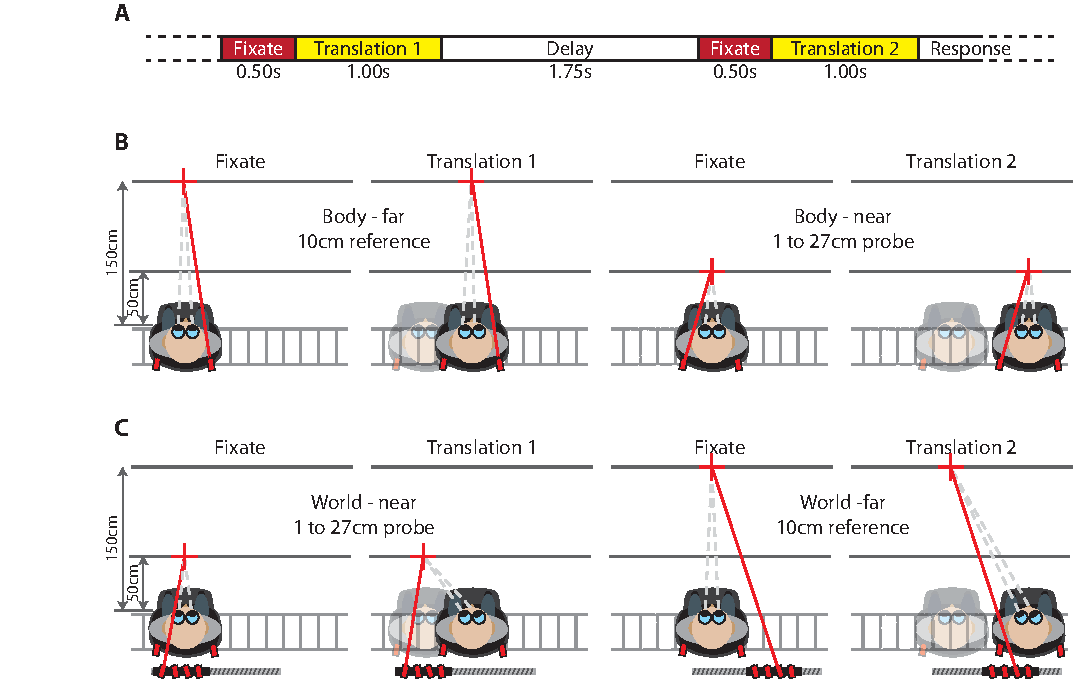
\includegraphics[width=1.0\textwidth]{src/paper4/p4_figure1.pdf}

    \caption{\panelref{A} Time course  of key events within a single trial. In each of the two intervals, a 0.50 \si{\second} fixation period (red) precedes the lateral translation (yellow). A 1.75 \si{\second} long delay period (shown in white) separates the two intervals. After the second translation, the participant responded whether this second translation was longer or shorter than the first. \panelref{B} and \panelref{C} Top-view illustrating key events in a far versus near body-fixed fixation trial (\panelref{B}) and a near versus far world-fixed fixation trial (\panelref{C}). The first panel shows the initial fixation to the target (red cross) followed by a translation in the second panel. The third panel shows the initial fixation before the second movement interval followed by a translation in the fourth panel.}
    \label{p4:fig1}    
\end{figure}
 
The timing of a single trial is shown in \figref{p4:fig1}A. Each trial started with the onset of a central fixation point (i.e. aligned between the eyes) for 0.5 \si{\second}. Subsequently, the first 1s motion interval commenced, during which the fixation type which was at on the two depths, remained stationary (world condition) or moved along with the participant (body condition). Subsequently a 1.75 \si{\second} delay followed in which the participant was kept in stationary complete darkness. Then, the central fixation point reappeared, followed 0.5 \si{\second} later by a second 1 \si{\second} translation interval, with the same fixation condition but with the fixation point at the other depth as in the first interval. Finally, the participant responded by moving a 1-dimensional joystick away from (longer) or towards (shorter) the body. Top-view illustrations of body-centered and world-centered trials are shown in \figref{p4:fig1} panels B and C.

\begin{table}
    \begin{tabular}{llll}
    Comparison & Reference & 1st interval & Direction \\
    \hline
    Body & Near & Reference & Right \\
    Near vs. far & & & Left \\    
    & & Probe & Right \\
    & & & Left \\
    \cline{2-4}
	& Far & Reference & Right \\
    & & & Left \\    
    & & Probe & Right \\
    & & & Left \\
    \hline
    World & Near & Reference & Right \\
    Near vs. far & & & Left \\    
    & & Probe & Right \\
    & & & Left \\
    \cline{2-4}
	& Far & Reference & Right \\
    & & & Left \\    
    & & Probe & Right \\
    & & & Left \\
    \end{tabular}

    \caption{List of the 2 main comparisons that we tested. The (10cm) reference movement was presented in either the first or the second interval. We also manipulated movement direction (leftward vs rightward) yielding a total of 16 trial types.}

    \label{p4:tab1}
\end{table}

% Should look at the 4 vs 16 in the next part, sounds confusing.
Across trials, we varied fixation distance of the reference and probe, giving a total of four variations per condition (see \tabref{p4:tab1}). Movement direction (either leftward or rightward) alternated between consecutive trials. The size of the probe translation was adaptively chosen based on the participants' earlier responses (Psi method; \citeNP{kontsevich1999}) to determine the point of subjective equality. This was done separately for all 16 trial types (2 main conditions x 2 reference stimuli x 2 reference/probe orders x 2 movement directions; see Table 1). A total of 25 trials were collected per trial type yielding a total of 200 trials for each of the two main conditions.

Trials were presented in two one-hour sessions. To prevent dark adaptation, we turned on the lights for 5 \si{\second} after each block of 8 trials, and for at least 30 s after every 2 blocks. Each of the 16 unique trial types were presented once every 2 blocks. After each block, the adaptive procedure determined which translation size to test in the following block. To increase the number of data-points available to the adaptive psychometric procedure at the beginning of the experiment, we collapsed across movement direction and reference order for the first 10 trials. After that, the procedure ran separately for each of the 16 distinct trial types.

\subsection{Data analysis}

For each combination of the two main conditions and the two reference/probe orders (see \tabref{p4:tab1}), we quantified the perceived probe translation by calculating the probability the probe translation was perceived longer than the reference translation as a function of actual probe translation. We used a maximum likelihood fit of a cumulative Gaussian function to summarize the psychometric data:

\begin{equation}
\label{p4:eq1}
P(x) = \lambda + (1 - 2\lambda) \frac{1}{\sigma \sqrt{2\pi}} \int_{-\infty}^{x}{e^{-(y-\mu)^2 / 2\sigma^2}}dy,
\end{equation}

in which $|x|$ represents the size of the probe translation. The mean of the Gaussian, PSE, represents the point of subjective equality. The slope of the curve reflects the precision ($1/\sigma$) of reference-probe discrimination performance. Parameter $\lambda$, representing the lapse rate, accounts for stimulus-independent errors caused by subject lapses or mistakes and was restricted to small values ($\lambda < 0.06$). Fits were performed using the Psignifit toolbox \cite{wichmann2001,wichmann2001b}.

For each trial type (see \tabref{p4:tab1}), we also quantified eye movements, corrected for drift based on initial fixation. We discarded trials containing blinks as well as trials in which final eye position exceeded two standard deviations from the condition's average. Based on these criteria, 12\% of all trials were discarded. Of the remaining trails, we computed the average ratio between the measured eye excursion, $\varphi_i$, and the angle that would be needed were the trial testing the world-fixed condition. The latter is computed by taking the arc-tangent of the actual translation distance, $m_i$, divided by the fixation depth, $d_i$, which for small $\varphi$ can be approximated by $g_c = \frac{\varphi_i m_i}{d_i}$. We computed this ratio, $g_c$, for every trial type $c$ (see \tabref{p4:tab1}). Ideally, for body-fixed trials, $g_c = 0$; and for world-fixed trials, $g_c = 1$.


\subsection{Model}

Using a straightforward model, we investigate to what extent fixation depth is taken into account in the contribution of eye movements to self-motion perception. As in \citeA{clemens2015a}, we model the perceived translation, $p_i$, as a weighted combination of a vestibular, $m_i$, and oculomotor estimate of translation, $\hat{\varphi}_i$ (\eqnref{p4:eq4}). 

\begin{equation}
\label{p4:eq4}
p_i = \alpha_{d_i} \hat{\varphi}_i + (1 - \alpha_{d_i}) m_i
\end{equation}

% This seems a bit flaky!
Variable $i$ represents either the reference, $r$, or probe, $p$, interval. Ideally, to server a veridical self-motion cue, the brain must scale the eye movement by the depth of fixation, $d$. This scaling is reflected by parameter, $\alpha_{d_i}$. If this parameter is the same across the two fixation depths, $d$, then there is no depth-dependent modulation of the oculomotor estimate of translation.

By definition, at the PSE, the probe translation is perceived as equal in length to the 10 cm reference translation, $p_r = p_p$. By substituting both sides by the right hand side of \eqnref{p4:eq4}, we then obtain:

\begin{equation}
\label{p4:eq5}
\alpha_{d_r} \hat{\varphi}_r + (1 - \alpha_{d_r}) m_r = \alpha_{d_p} \hat{\varphi}_p + (1 - \alpha_{d_p}) m_p + \epsilon
\end{equation}

We fit \eqnref{p4:eq5} to the data using linear regression, finding one weight for every fixation depth (that is, $\alpha_{50}$ and $\alpha_{200}$) that minimizes the sum of squared errors ($\Sigma \epsilon^2$). Because these parameters can, in theory, contain both a depth-dependent and a depth-independent scaling, we compute their ratio, $\frac{\alpha_{200}}{\alpha_{50}}$, to remove any depth independent components. In case of perfect compensation, the expected ratio is $\frac{200}{50} = 4$, while in case of no depth-dependent scaling it is 1.
